\documentclass[tikz,border=2pt]{standalone}
\usepackage{amsmath}
\usepackage{pgfplots}
\pgfplotsset{compat=1.18}

\begin{document}
% sin x ~ x as x -> 0: the two graphs become indistinguishable near 0 because their ratio tends to 1,
% even though they separate further away.
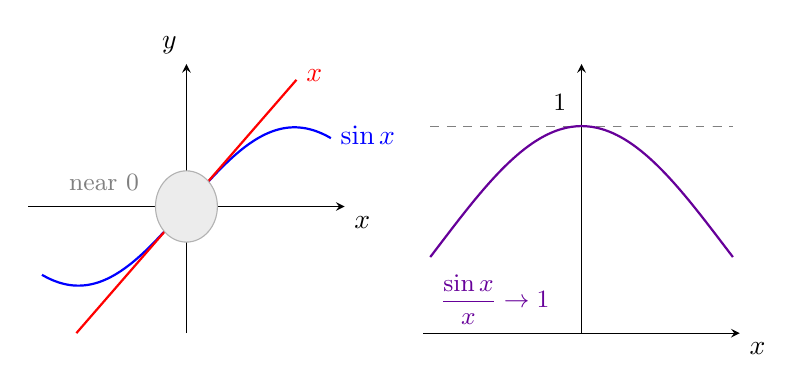
\begin{tikzpicture}
	\begin{axis}[
		name=left,
		axis lines=middle,
		xmin=-2.3, xmax=2.3,
		ymin=-1.6, ymax=1.8,
		xtick=\empty, ytick=\empty,
		xlabel={$x$}, ylabel={$y$},
		xlabel style={below right}, ylabel style={above left},
		samples=150, smooth, clip=false,
		width=5.6cm, height=5cm
		]
		\addplot[thick, blue, domain=-2.1:2.1] {sin(deg(x))};
		\addplot[thick, red, domain=-1.6:1.6] {x};
		\node[blue, anchor=west] at (axis cs:2.1,0.9) {$\sin x$};
		\node[red, anchor=west] at (axis cs:1.6,1.65) {$x$};
		\draw[gray!60, fill=gray!15] (axis cs:0,0) circle [radius=0.45];
		\node[gray, anchor=east, font=\small] at (axis cs:-0.55,0.3) {near $0$};
	\end{axis}
	\begin{axis}[
		at={(left.east)}, anchor=west, xshift=1cm,
		axis lines=middle,
		xmin=-2.3, xmax=2.3,
		ymin=0, ymax=1.3,
		xtick=\empty, ytick=\empty,
		xlabel={$x$}, ylabel={},
		xlabel style={below right},
		samples=150, smooth, clip=false,
		width=5.6cm, height=5cm
		]
		\addplot[gray, dashed, domain=-2.2:2.2] {1};
		\addplot[thick, blue!60!red, domain=-2.2:2.2] {sin(deg(x))/x};
		\node[anchor=south east, font=\small] at (axis cs:-0.08,1.03) {$1$};
		\node[blue!60!red, anchor=west, font=\small] at (axis cs:-2.2,0.16) {$\dfrac{\sin x}{x}\to 1$};
	\end{axis}
\end{tikzpicture}
\end{document}
